% !TEX encoding = UTF-8 Unicode
%!TEX root = thesis.tex
% !TEX spellcheck = en-US
%%=========================================
\section{Experiment 5}
This experiment is about combining several audio effects in serial and parallel. The idea is that this allows for altering the sound in more ways than with only a single audio effect. The hypothesis is that a genetic algorithm could be adept at choosing which effects to use and how. This experiment will study two different effect networks, as illustrated by figure \ref{TODO} and \ref{TODO}. From now on, they will be referred to as ``1 layer'' and ``2 layers'', respectively. In addition, to get an idea of how each effect performs individually, the effects used will be tested separately.

\begin{figure}[h]
    \centering
    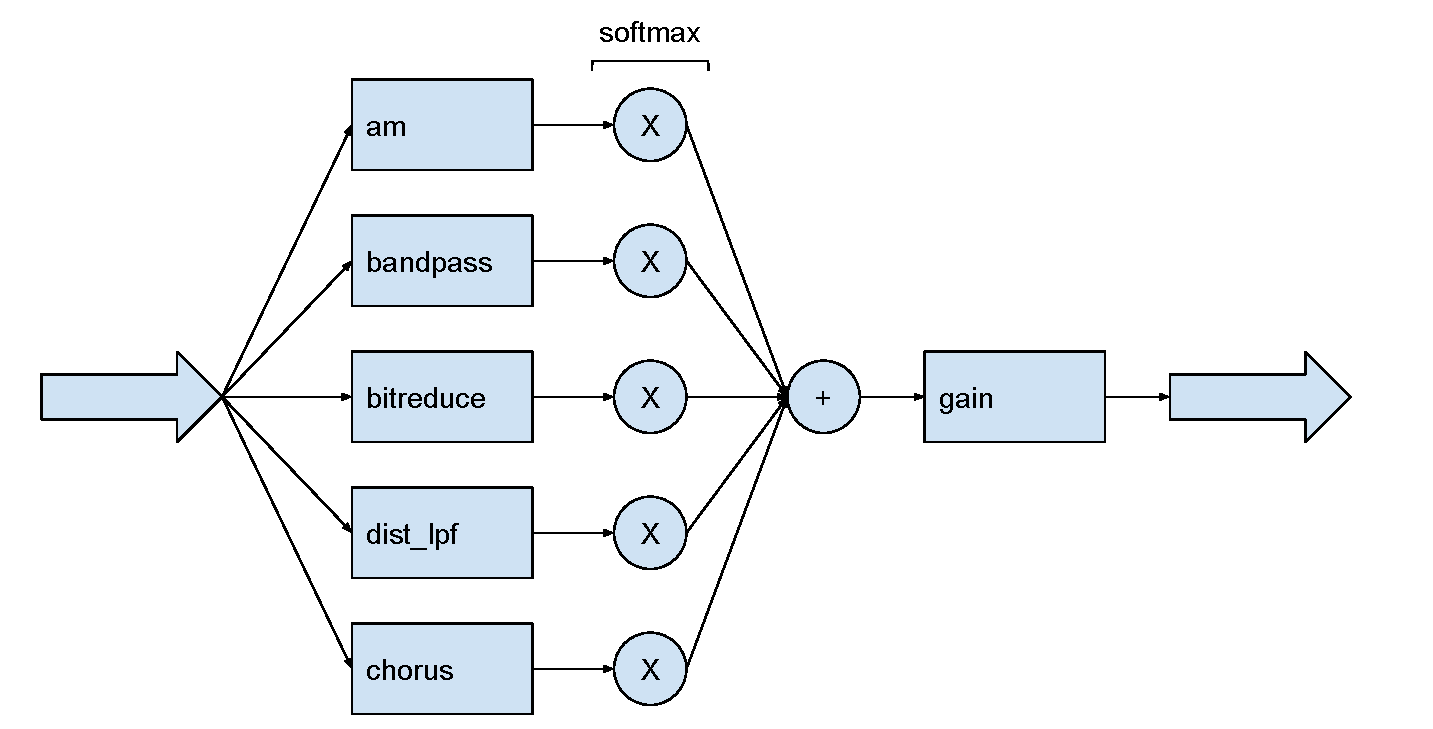
\includegraphics[width=0.75\textwidth]{exp5_1layer_flow}
    \caption{Signal flow in the ``1 layer'' configuration}
    \label{fig:exp5_1layer_flow}
\end{figure}

\begin{figure}[h]
    \centering
    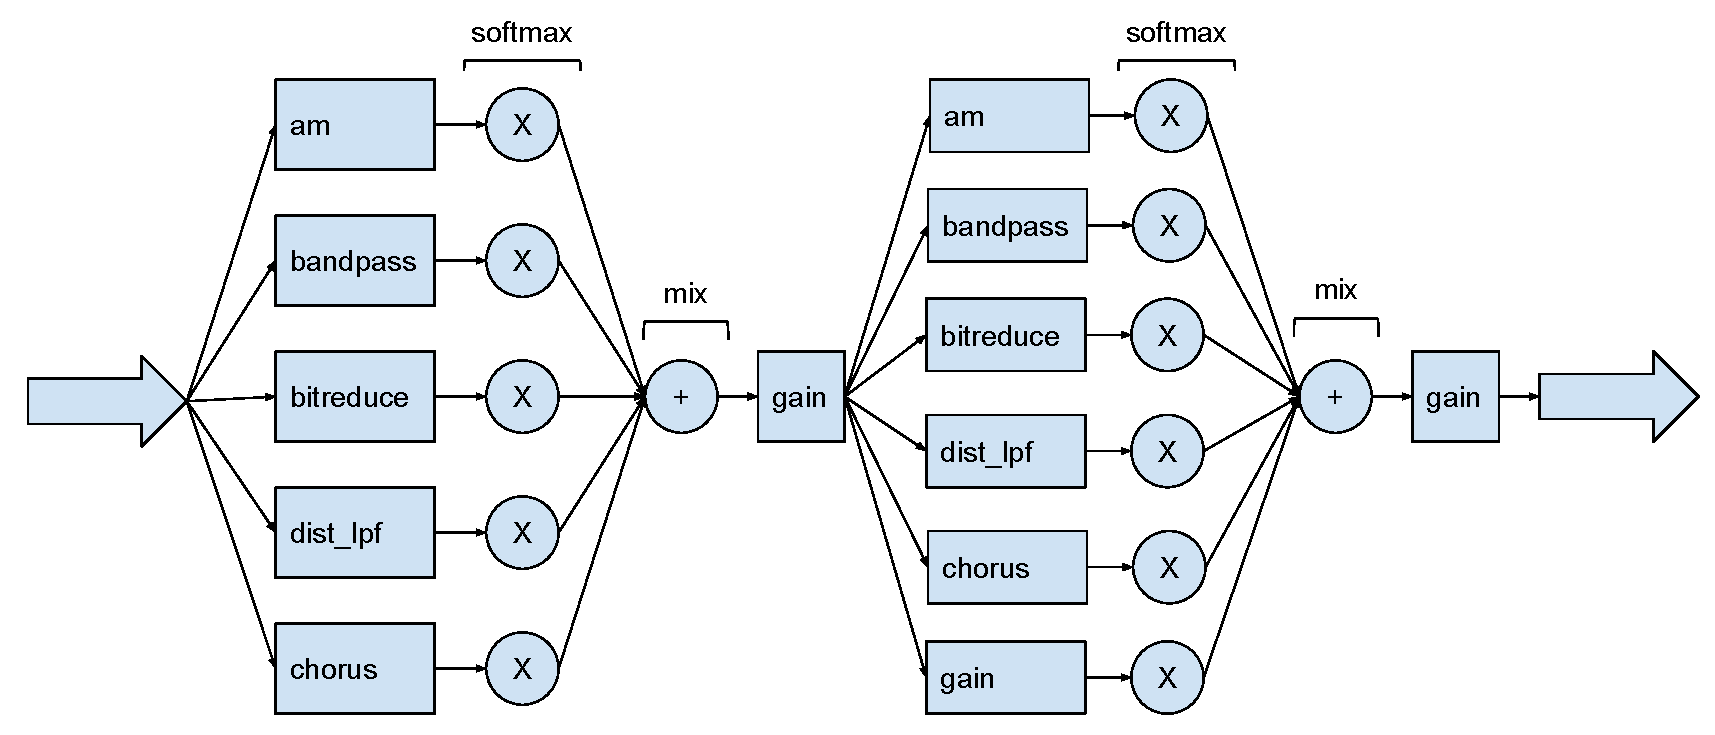
\includegraphics[width=0.99\textwidth]{exp5_2layers_flow}
    \caption{Signal flow in the ``2 layers'' configuration}
    \label{fig:exp5_2layers_flow}
\end{figure}

For baseline performance measure, each effect has been tested separately. Then they were run in parallel TODO



In this experiment, we do 5 fx in parallel => ok result
am
band-pass
bitreduce
dist lpf
chorus

(Then 2 layers of 5?)
Then 10 fx in parallel => bad result

Suggest pre-training with each fx separately, then training the mix
Softmax mixing may also be bad -> suggest independent mix values

create video demonstrating 1st successful result here

Say something about hypothesis about which fx will be used. Which ones were actually used? Do the same for parameters. Show mix values in horizon graph. Say that am and chorus make sound richer, while we need it filtered.

\begin{figure}[h]
    \centering
    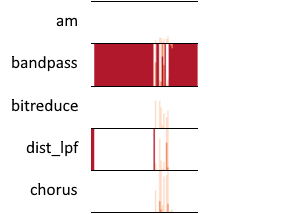
\includegraphics[width=0.45\textwidth]{exp5_1layer_softmax}
    \caption{Gain values for each effect in the best result with configuration 1 TODO}
    \label{fig:exp5_1layer_softmax}
\end{figure}

\begin{figure}[h]
    \centering
    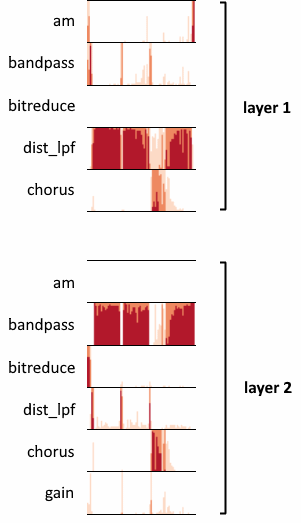
\includegraphics[width=0.45\textwidth]{exp5_2layers_softmax}
    \caption{Gain values for each effect in the best result with configuration 2 TODO}
    \label{fig:exp5_2layers_softmax}
\end{figure}

\begin{figure}[h]
    \centering
    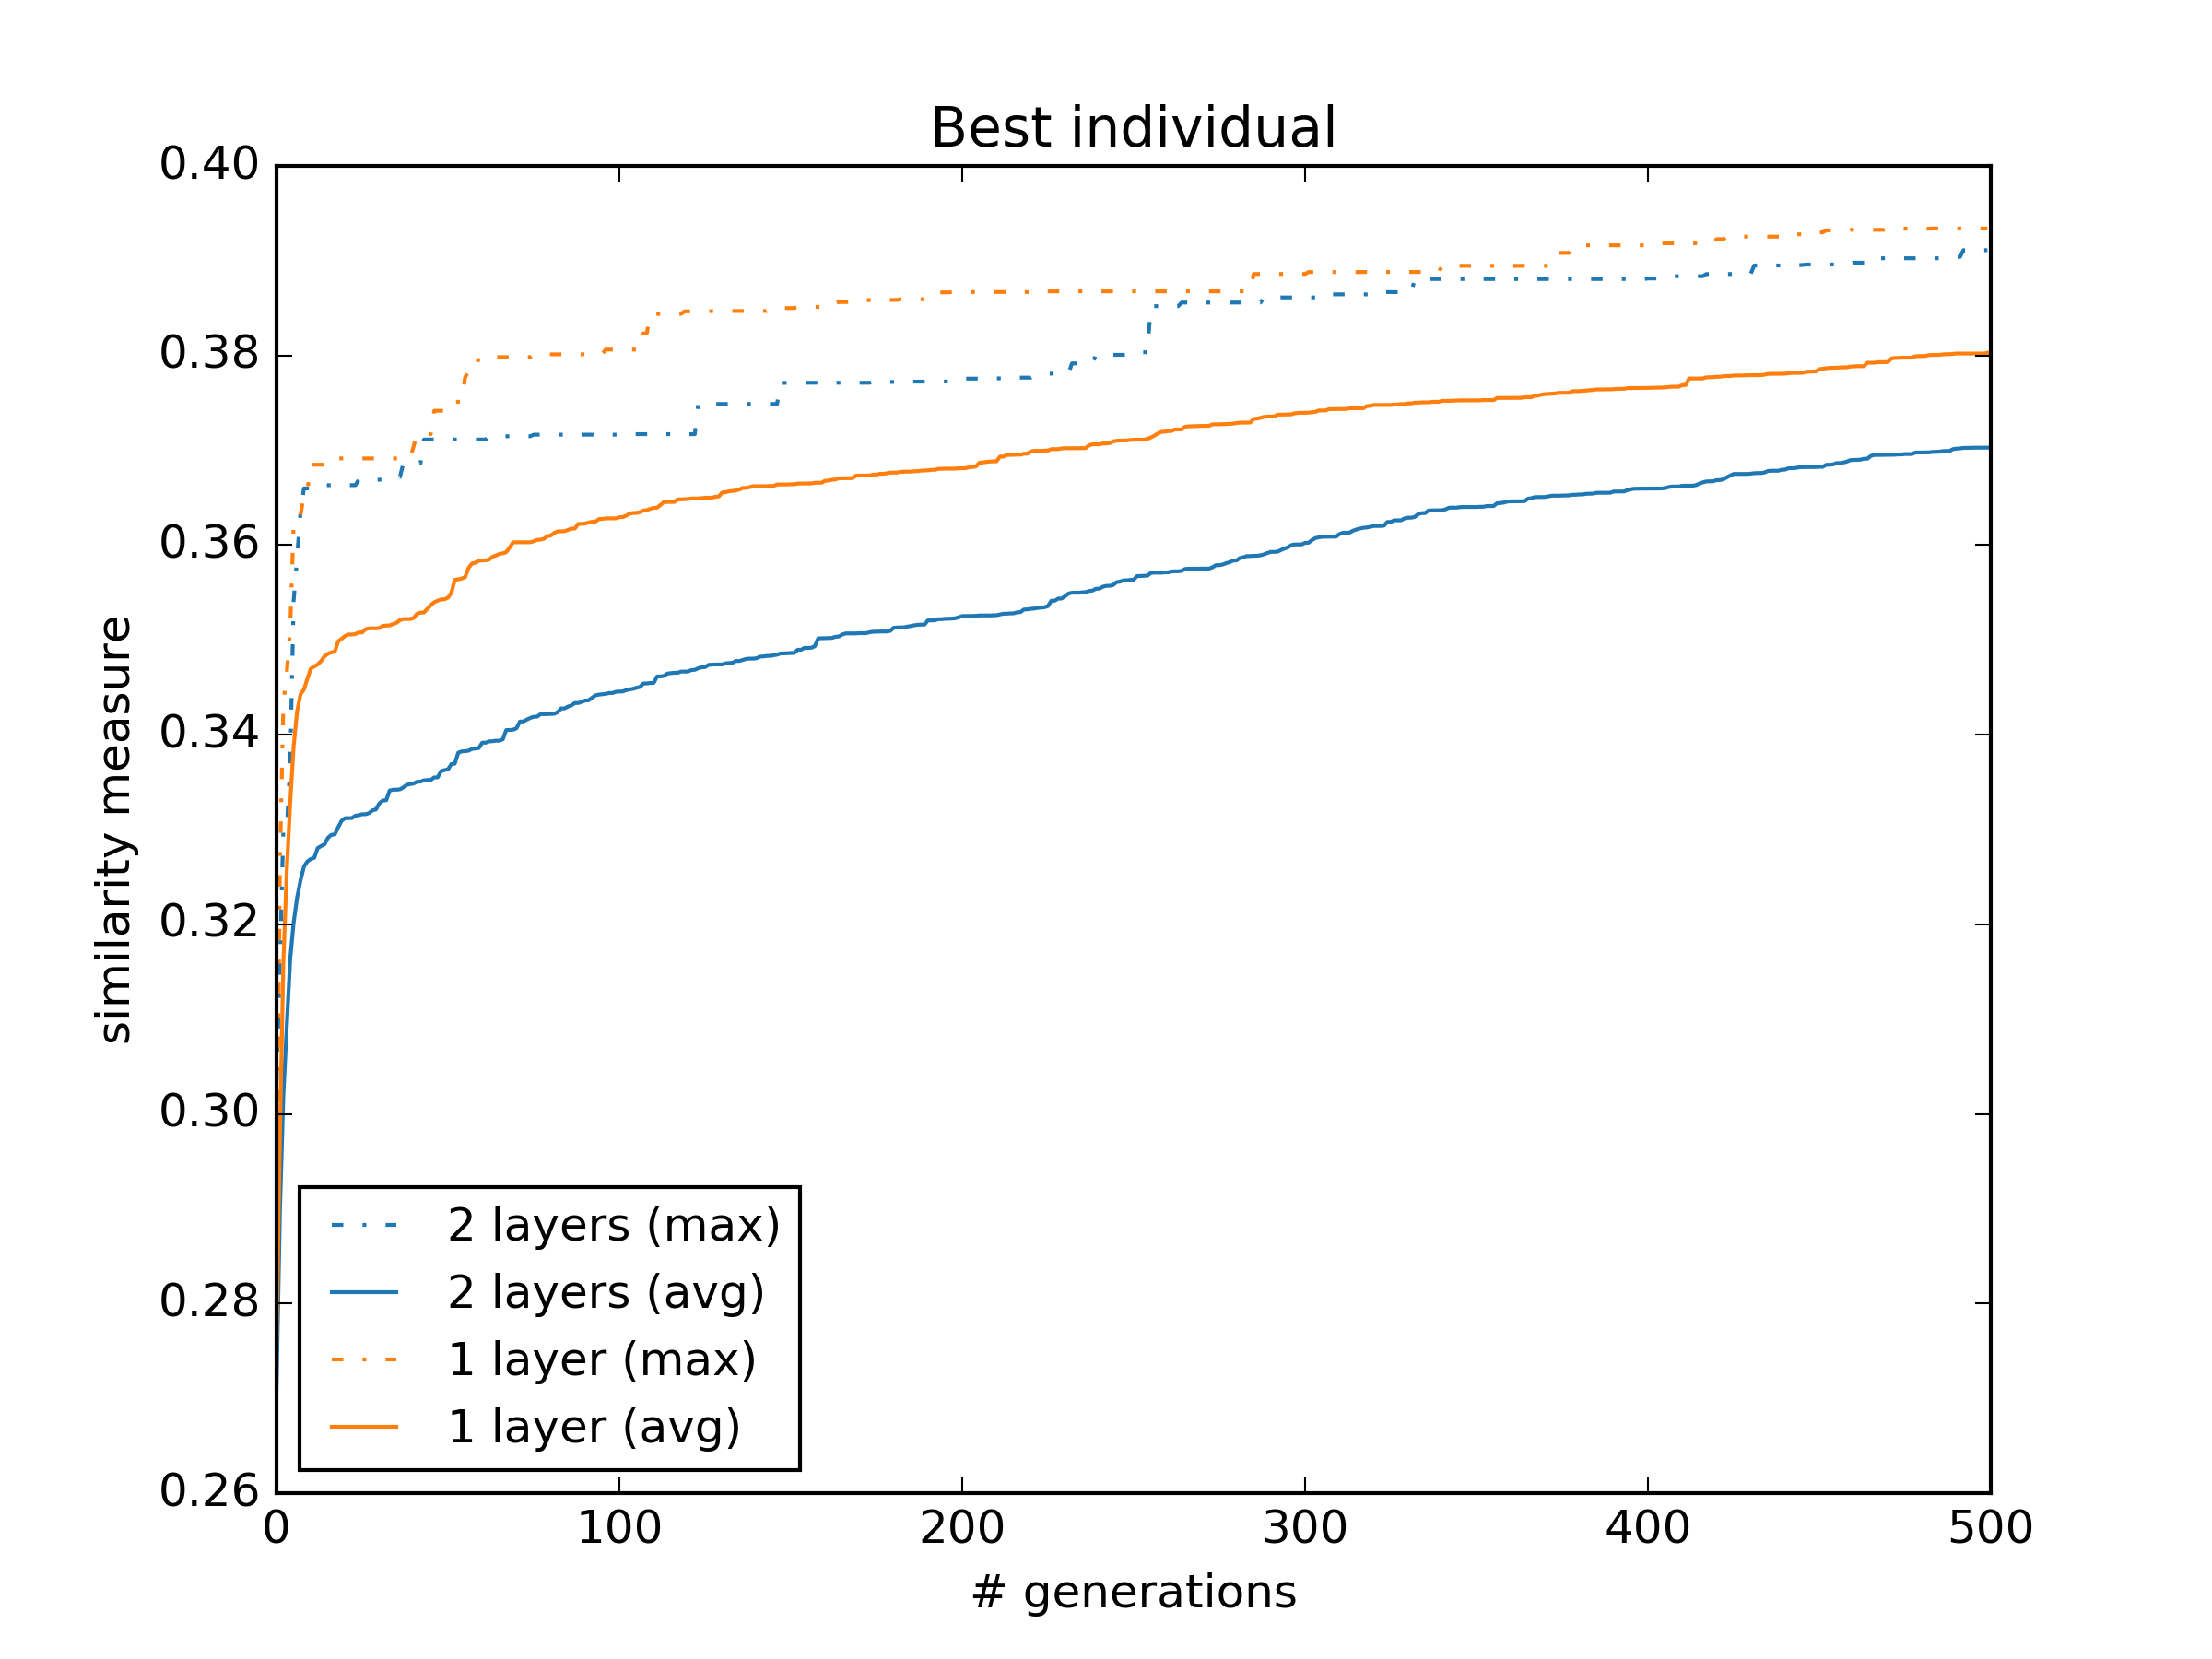
\includegraphics[width=0.99\textwidth]{exp5_avg_max}
    \caption{Aggregated fitness values}
    \label{fig:exp5_avg_max}
\end{figure}

\begin{figure}[h]
    \centering
    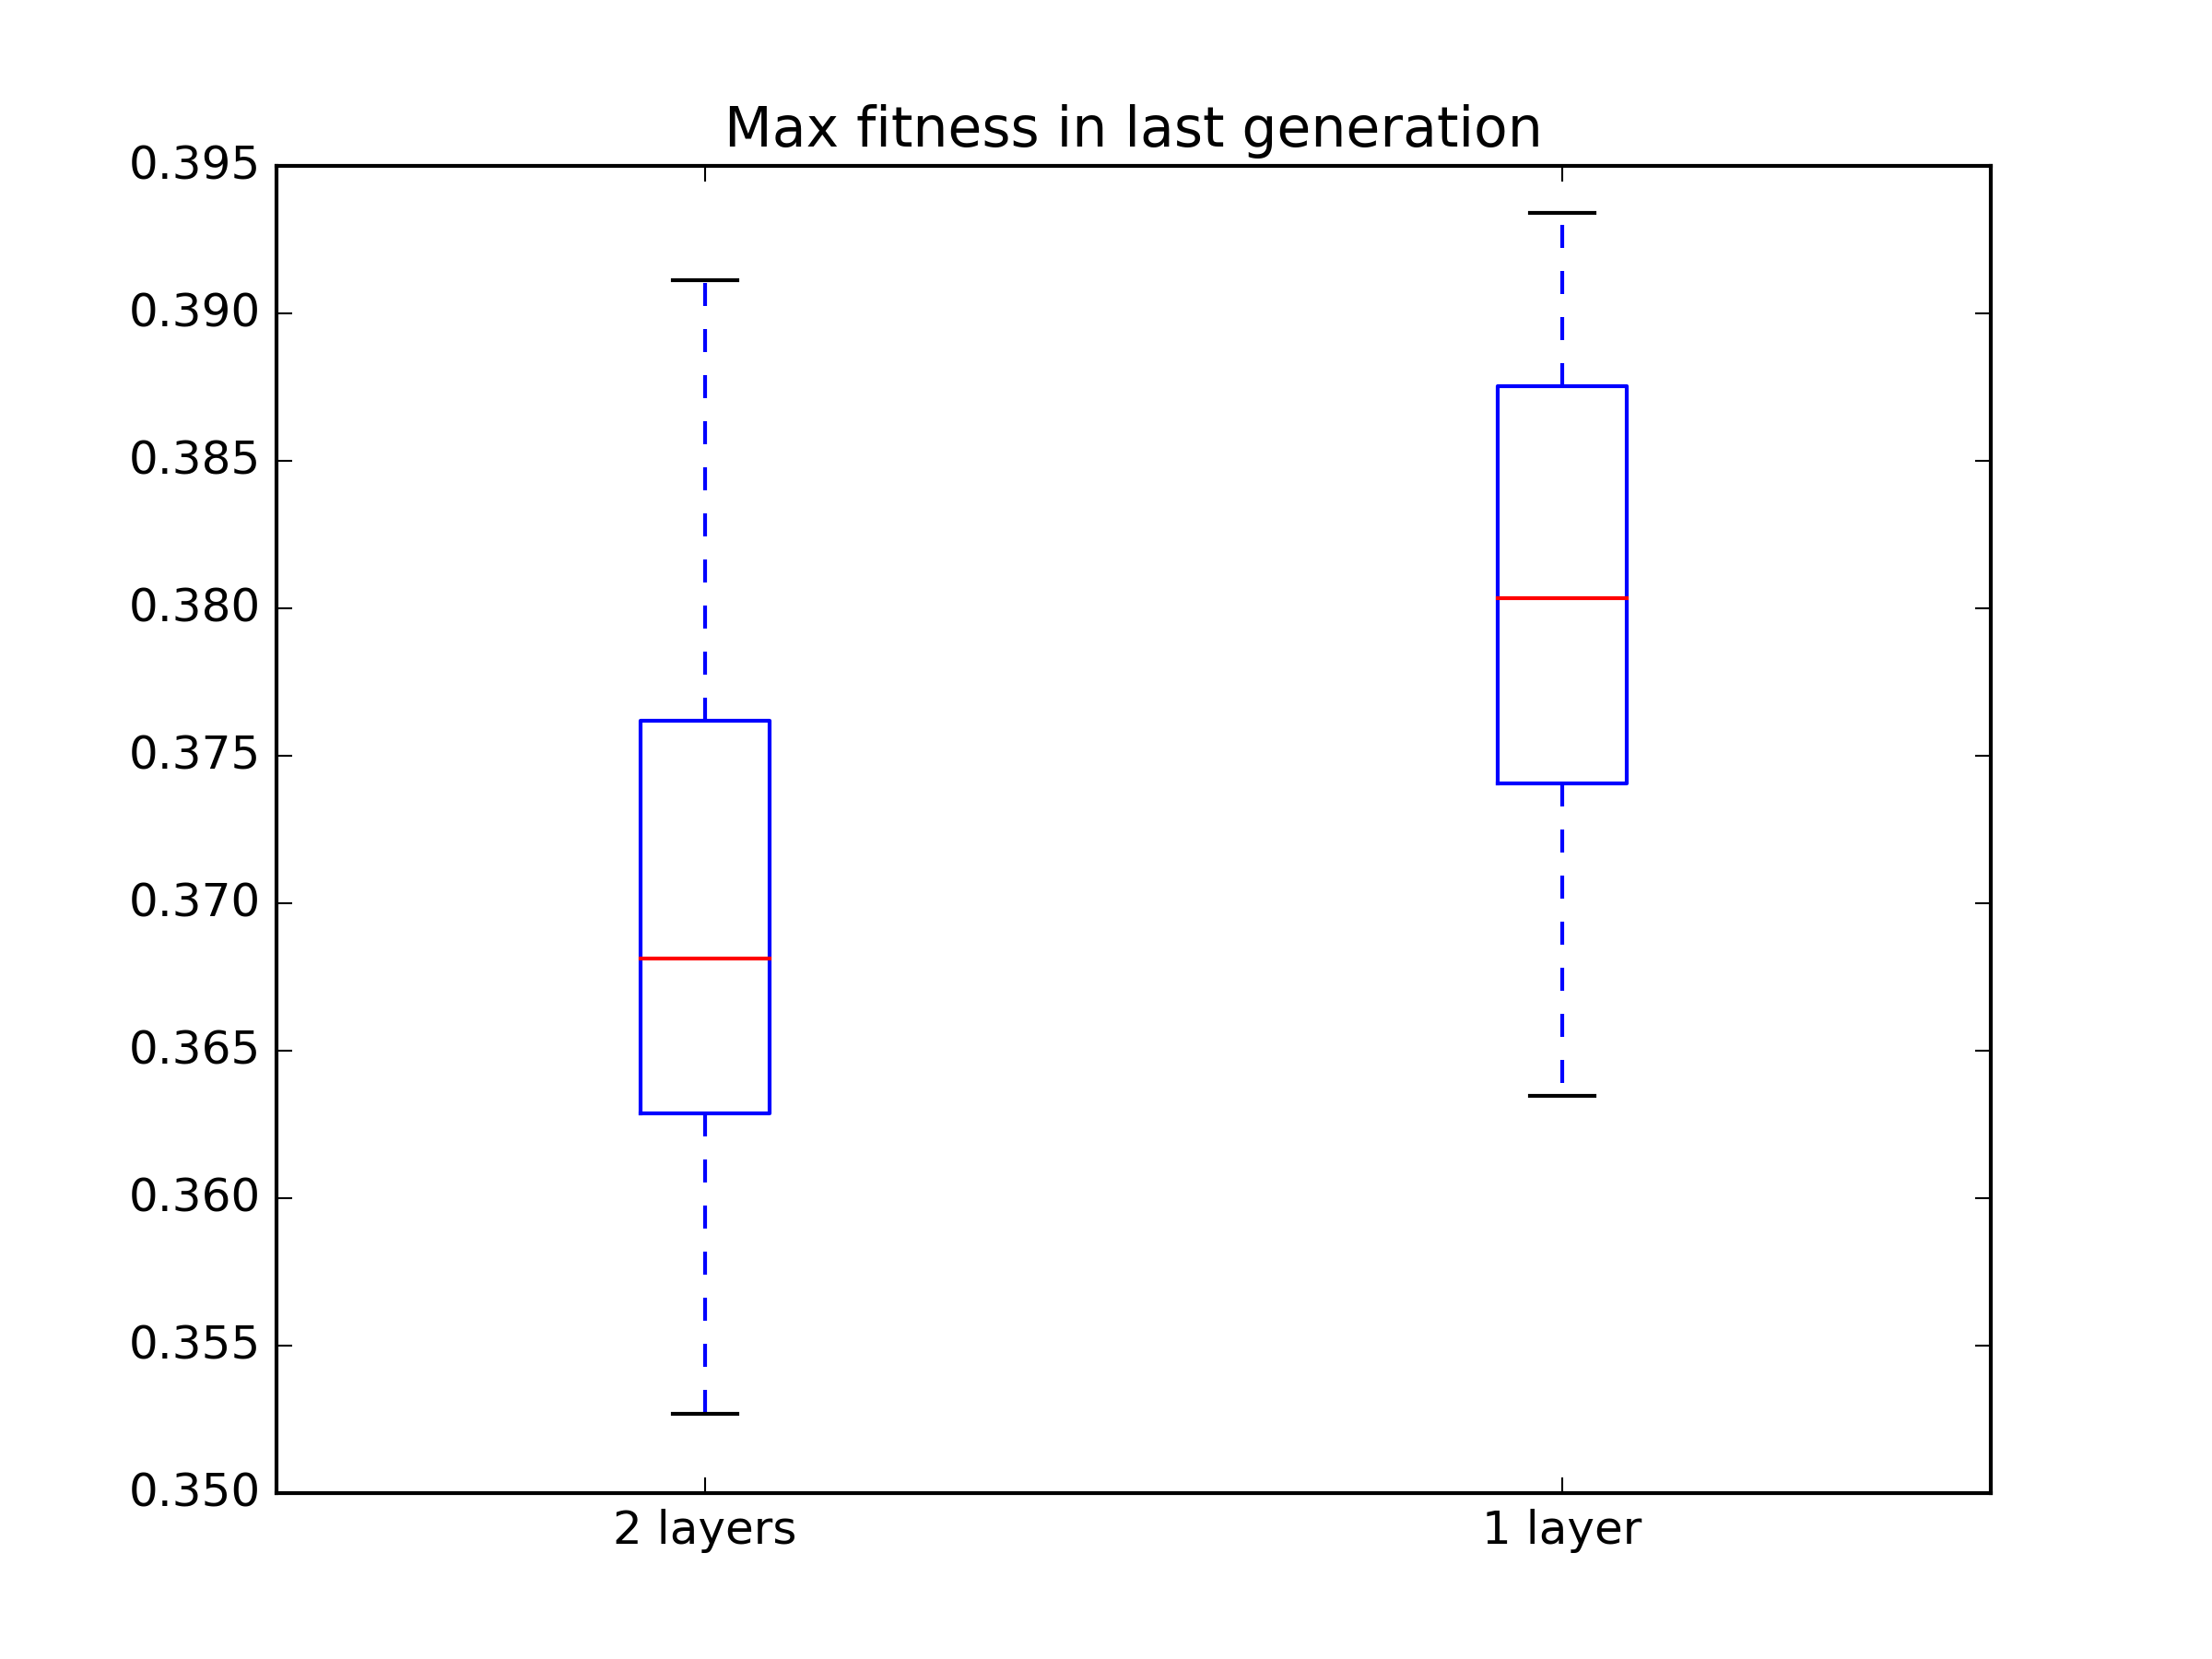
\includegraphics[width=0.99\textwidth]{exp5_box}
    \caption{Box-and-whiskers plot of fitness values in the last generation}
    \label{fig:exp5_box}
\end{figure}
